\documentclass[10pt,a4paper]{ctexart}
\usepackage[margin=2cm]{geometry}
\usepackage{graphicx}
\usepackage{float}      % 支持 [H] 浮动体选项
\usepackage{hyperref}
\usepackage{amsmath}    % 提供方程环境
\usepackage{physics}    % 简化向量、微分算子语法
\newcommand{\myspace}[1]{\par\vspace{#1\baselineskip}} %自定义空一行
\usepackage{fancyhdr}
\usepackage{booktabs}
\usepackage{tabularx}
\usepackage{array}  % 提供更多列类型
\usepackage{subfig}
\usepackage{siunitx}
\pagestyle{fancy}
\fancyhf{}  % 清除所有页眉页脚
\fancyfoot[C]{\thepage}  % 在页脚中央设置页码
\renewcommand{\headrulewidth}{0pt}  % 去掉页眉横线
\renewcommand{\footrulewidth}{0pt}  % 去掉页脚横线

\usepackage{hyperref}
\hypersetup{
    colorlinks=true,
    linkcolor=blue,
    filecolor=magenta,      
    urlcolor=cyan,
    pdftitle={Overleaf Example},
    pdfpagemode=FullScreen,
    }

\usepackage{titlesec}

% 重新定义section格式
\titleformat{\section}
  {\normalfont\Large\bfseries}
  {\chinese{section}、}
  {0pt}
  {}

% 给出常用字号的自定义指令
\newcommand{\chuhao}{\fontsize{42pt}{48pt}\selectfont}
\newcommand{\xiaochu}{\fontsize{36pt}{42pt}\selectfont}
\newcommand{\xiaoer}{\fontsize{18pt}{21.6pt}\selectfont}
\newcommand{\sanhao}{\fontsize{16pt}{20pt}\selectfont}
\newcommand{\xiaosan}{\fontsize{15pt}{18pt}\selectfont}
\newcommand{\sihao}{\fontsize{14pt}{18pt}\selectfont}
\newcommand{\xiaosi}{\fontsize{12pt}{16pt}\selectfont}
\newcommand{\wuhao}{\fontsize{10.5pt}{12.6pt}\selectfont}

% 定义中文数字转换
\titleformat{\section}
  {\normalfont\Large\bfseries}
  {\zhnum{section}、}  % 使用\zhnum而不是\chinese
  {0pt}
  {}

% 标题设置
\title{\xiaochu\textbf{物理实验报告}}
\author{}
\date{}

\begin{document}

\vspace*{36pt} % 顶部空白

% 居中填写区域
\begin{center}
    
\includegraphics[width = 9cm]{figure/head.png}
    
    \xiaochu\textbf{物理实验报告}
    % 预留空白区域
    \vspace{13pt}
    \vspace{13pt}
    \vspace{13pt}
    \vspace{13pt}
    
    \sanhao\textbf{实验名称：\underline{\makebox[10cm]{ 万用表的设计}}} \\[10pt]
    \sanhao\textbf{实验桌号：\underline{\makebox[10cm]{ 15}}} \\[10pt]
    \sanhao\textbf{指导教师：\underline{\makebox[10cm]{ 唐浩原 }}} \\[30pt]
    
    % 预留空白区域
    \myspace{6}
    
   \sihao\textbf{班级：\underline{\makebox[6cm]{}}} \\[10pt]
   \sihao\textbf{姓名：\underline{\makebox[6cm]{}}} \\[10pt]
    \sihao\textbf{学号：\underline{\makebox[6cm]{}}} \\[30pt]
    
   \sihao\textbf{实验日期: 
   \underline{\makebox[0.8cm]{2026}}  年 
   \underline{\makebox[0.4cm]{1}}月
   \underline{\makebox[0.4cm]{5}}日  
   星期\underline{\makebox[0.6cm]{三}}上午}
    
    \vspace{18pt}
    \sihao 浙江大学物理实验教学中心
    
\end{center}

\newpage

\section{预习报告}

    \subsection{实验综述}
    
    \xiaosi （自述实验现象、实验原理和实验方法，不超过300字，5分）
 
    本实验主要包括电表内阻测量及电表改装两部分内容。首先采用替代法和中值法精确测定微安表的内阻，这是后续电表改装的基磁基础。随后进行电表量程扩展：通过在表头两端并联适当的分流电阻，可将微安表改装为毫安表或安培表；而在表头上串联合适的分压电阻，则可将其改装为伏特表。最后，利用改装的电流表配合电源和调零电阻构成欧姆表，用以测量未知电阻。当欧姆表示数为$I_x$时，设其等效内阻为$R_0$，电源电动势为$E$，根据闭合电路欧姆定律可得：
$$ E = I_x(R_0 + R_x) $$
由此解得待测电阻值为$R_x = \dfrac{E}{I_x} - R_0$。整个实验过程需注重注重电路连接的正确性及数据的准确记录与分析。
\myspace{2}
    \myspace{2}
    
    
    \subsection{实验重点}
    
    \xiaosi（简述本实验的学习重点，不超过100字，3分）
    
掌握电表内阻测量的替代法与中值法原理，理解电表改装的电路设计方法。学会计算分流电阻和分压电阻的阻值，完成电流表和电压表的改装。理解欧姆表的测量原理，能够分析改装后电表的刻度特性及测量误差来源。
    \myspace{2}
    
    \subsection{实验难点}
    
    \xiaosi（简述本实验的实现难点，不超过100字，2分）

电表内阻的精确测量是首要难点，需注意测量过程中对表头的保护。分流电阻和分压电阻的计算与选取要求精准，否则会引入较大系统误差。欧姆表中值电阻的确定及刻度非线性的补偿也是实际操作中的技术难点。
\myspace{2}
\section{原始数据}

    \xiaosi （将有老师签名的“自备数据记录草稿纸”的扫描或手机拍摄图粘贴在下方，20分）
   
\begin{figure}[H]
    \centering
    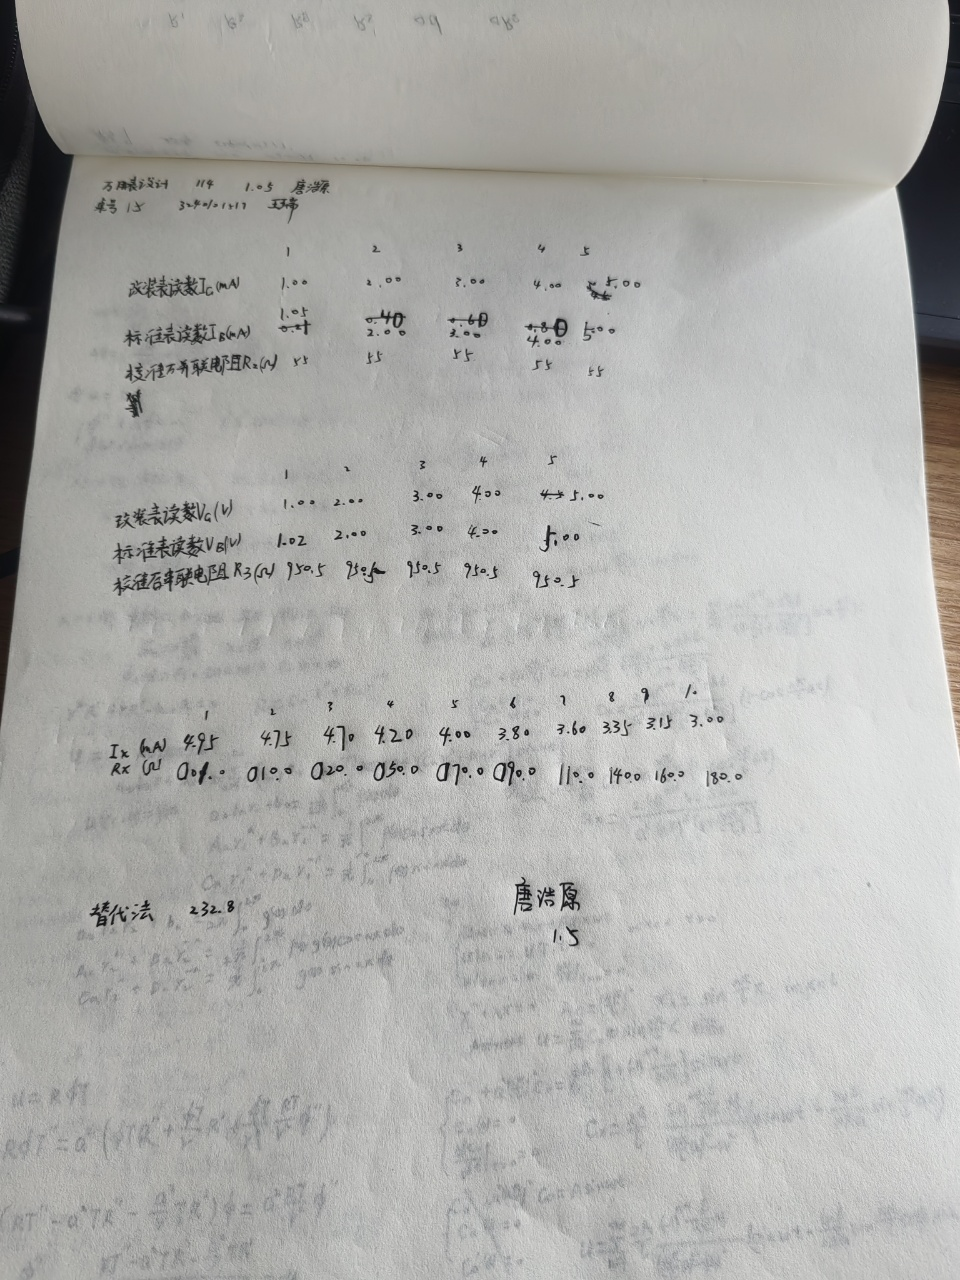
\includegraphics[width=0.8\textwidth]{figure/raw_data.jpg}
    \caption{原始数据记录}
\end{figure}
\section{结果与分析}

    \subsection{数据处理与结果}
    \xiaosi （列出数据表格、选择数据处理方法、给定测量或计算结果，30分）

\subsubsection{测量电流计的内阻}
通过替代法，测得电流计内阻为$R_g = 232.8 \Omega$。
\subsubsection{设计、改装并校准电流表}
经计算，$R_1 = 58.2\Omega$。由于电流表内阻测量误差，需要校准。根据电流表满偏时进行校准，电阻更新为$55\Omega$。实验数据如所示
\begin{table}[H]
  \centering
  \caption{改装5mA电流表的实验数据}
  \begin{tabular}{ccccccc}  % 添加了列格式：7个居中对齐的列
    \toprule
    实验序号 & 1 & 2 & 3 & 4 & 5 \\
    \midrule
    改装表读数$I_{\text{G}} / \si{\milli\ampere}$ & 1.00 & 2.00 & 3.00 & 4.00 & 5.00 \\
    \midrule
    标准表读数$I_{\text{B}} / \si{\milli\ampere}$ & 1.05 & 2.00 & 3.00 & 4.00 & 5.00 \\
    \midrule
    校准后的并联电阻$R_2 / \si{\ohm}$ & 55 & 55 & 55 & 55 & 55 \\
    \bottomrule
  \end{tabular}
  \label{tableA} % label label 要放在 caption 后面
\end{table}
最大绝对误差是$\Delta_{max} = \max|I_G - I_B| = 0.05 \si{\milli\ampere}$。
量程是5mA，因此改装电流表等级为$\frac{0.05}{5} \times 100\% = 1.0\%$，改装电流表等级为1.0.

改装后电流表的$I_G-I_B$曲线如所示
\begin{figure}[H]
  \centering
  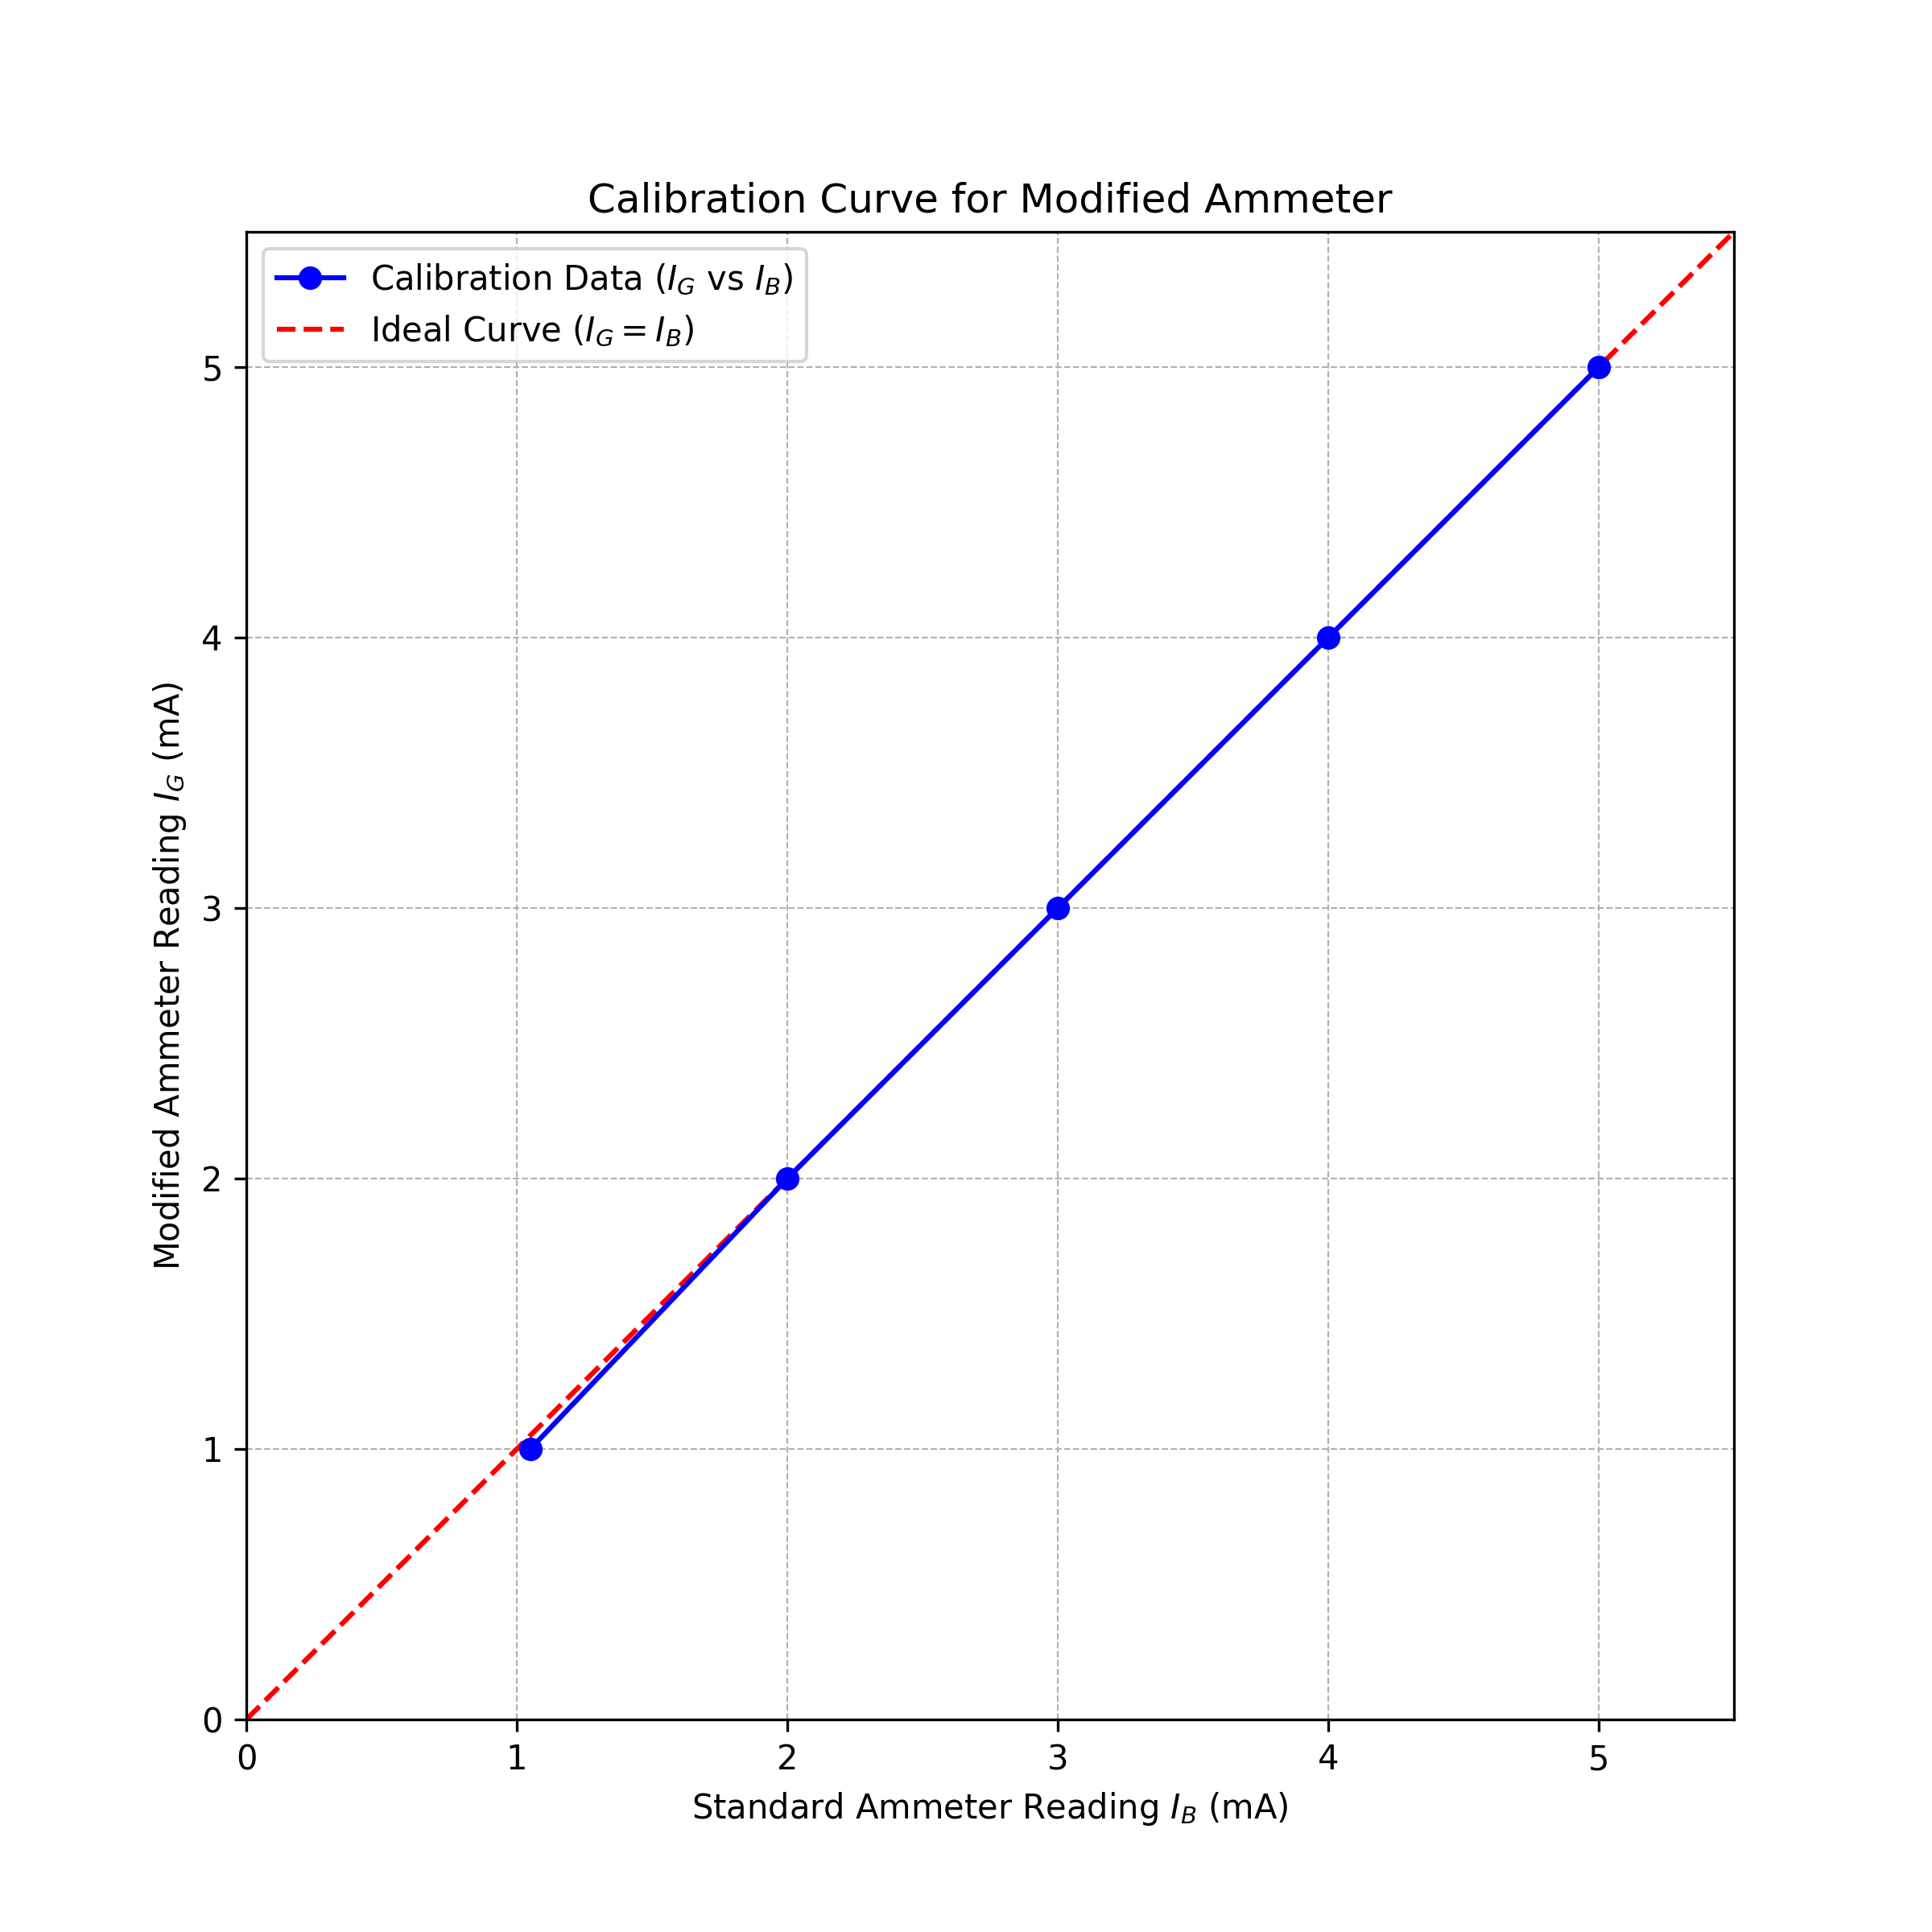
\includegraphics[width=0.4\textwidth]{figure/I.png}
  \caption{改装电流表的$I_G-I_B$曲线}
  \label{graphA}
\end{figure}

\subsubsection{设计、改装并校准电压表}
经计算，$R_3 = 950.5\Omega$。由于电压表内阻测量误差，需要校准。根据电压表满偏时进行校准，电阻更新为$950.0 \Omega$。实验数据如所示
\begin{table}[H]
  \centering
  \caption{改装{5}{V}电压表的实验数据}
  \begin{tabular}{ccccccc}
    \toprule
    实验序号 & 1 & 2 & 3 & 4 & 5 \\
    \midrule
    改装表读数$V_{\text{G}} / {V}$ & 1.00 & 2.00 & 3.00 & 4.00 & 5.00 \\
    \midrule
    标准表$V_{\text{B}} / {V}$ & 1.02 & 2.00 & 3.00 & 4.00 & 5.00 \\
    \midrule
    校准后的串联电阻$R_3 {}$ & 950.5 & 950.5 & 950.5 & 950.5 & 950.5 \\
    \bottomrule
    \label{tableV}
  \end{tabular}
\end{table}
计算得电压表等级为$ \left| \frac{0.02}{5}\right| = 0.4\%$，故改装电压表的等级为0.5。

改装后电压表的$V_G-V_B$曲线如所示。
\begin{figure}[H]
  \centering
  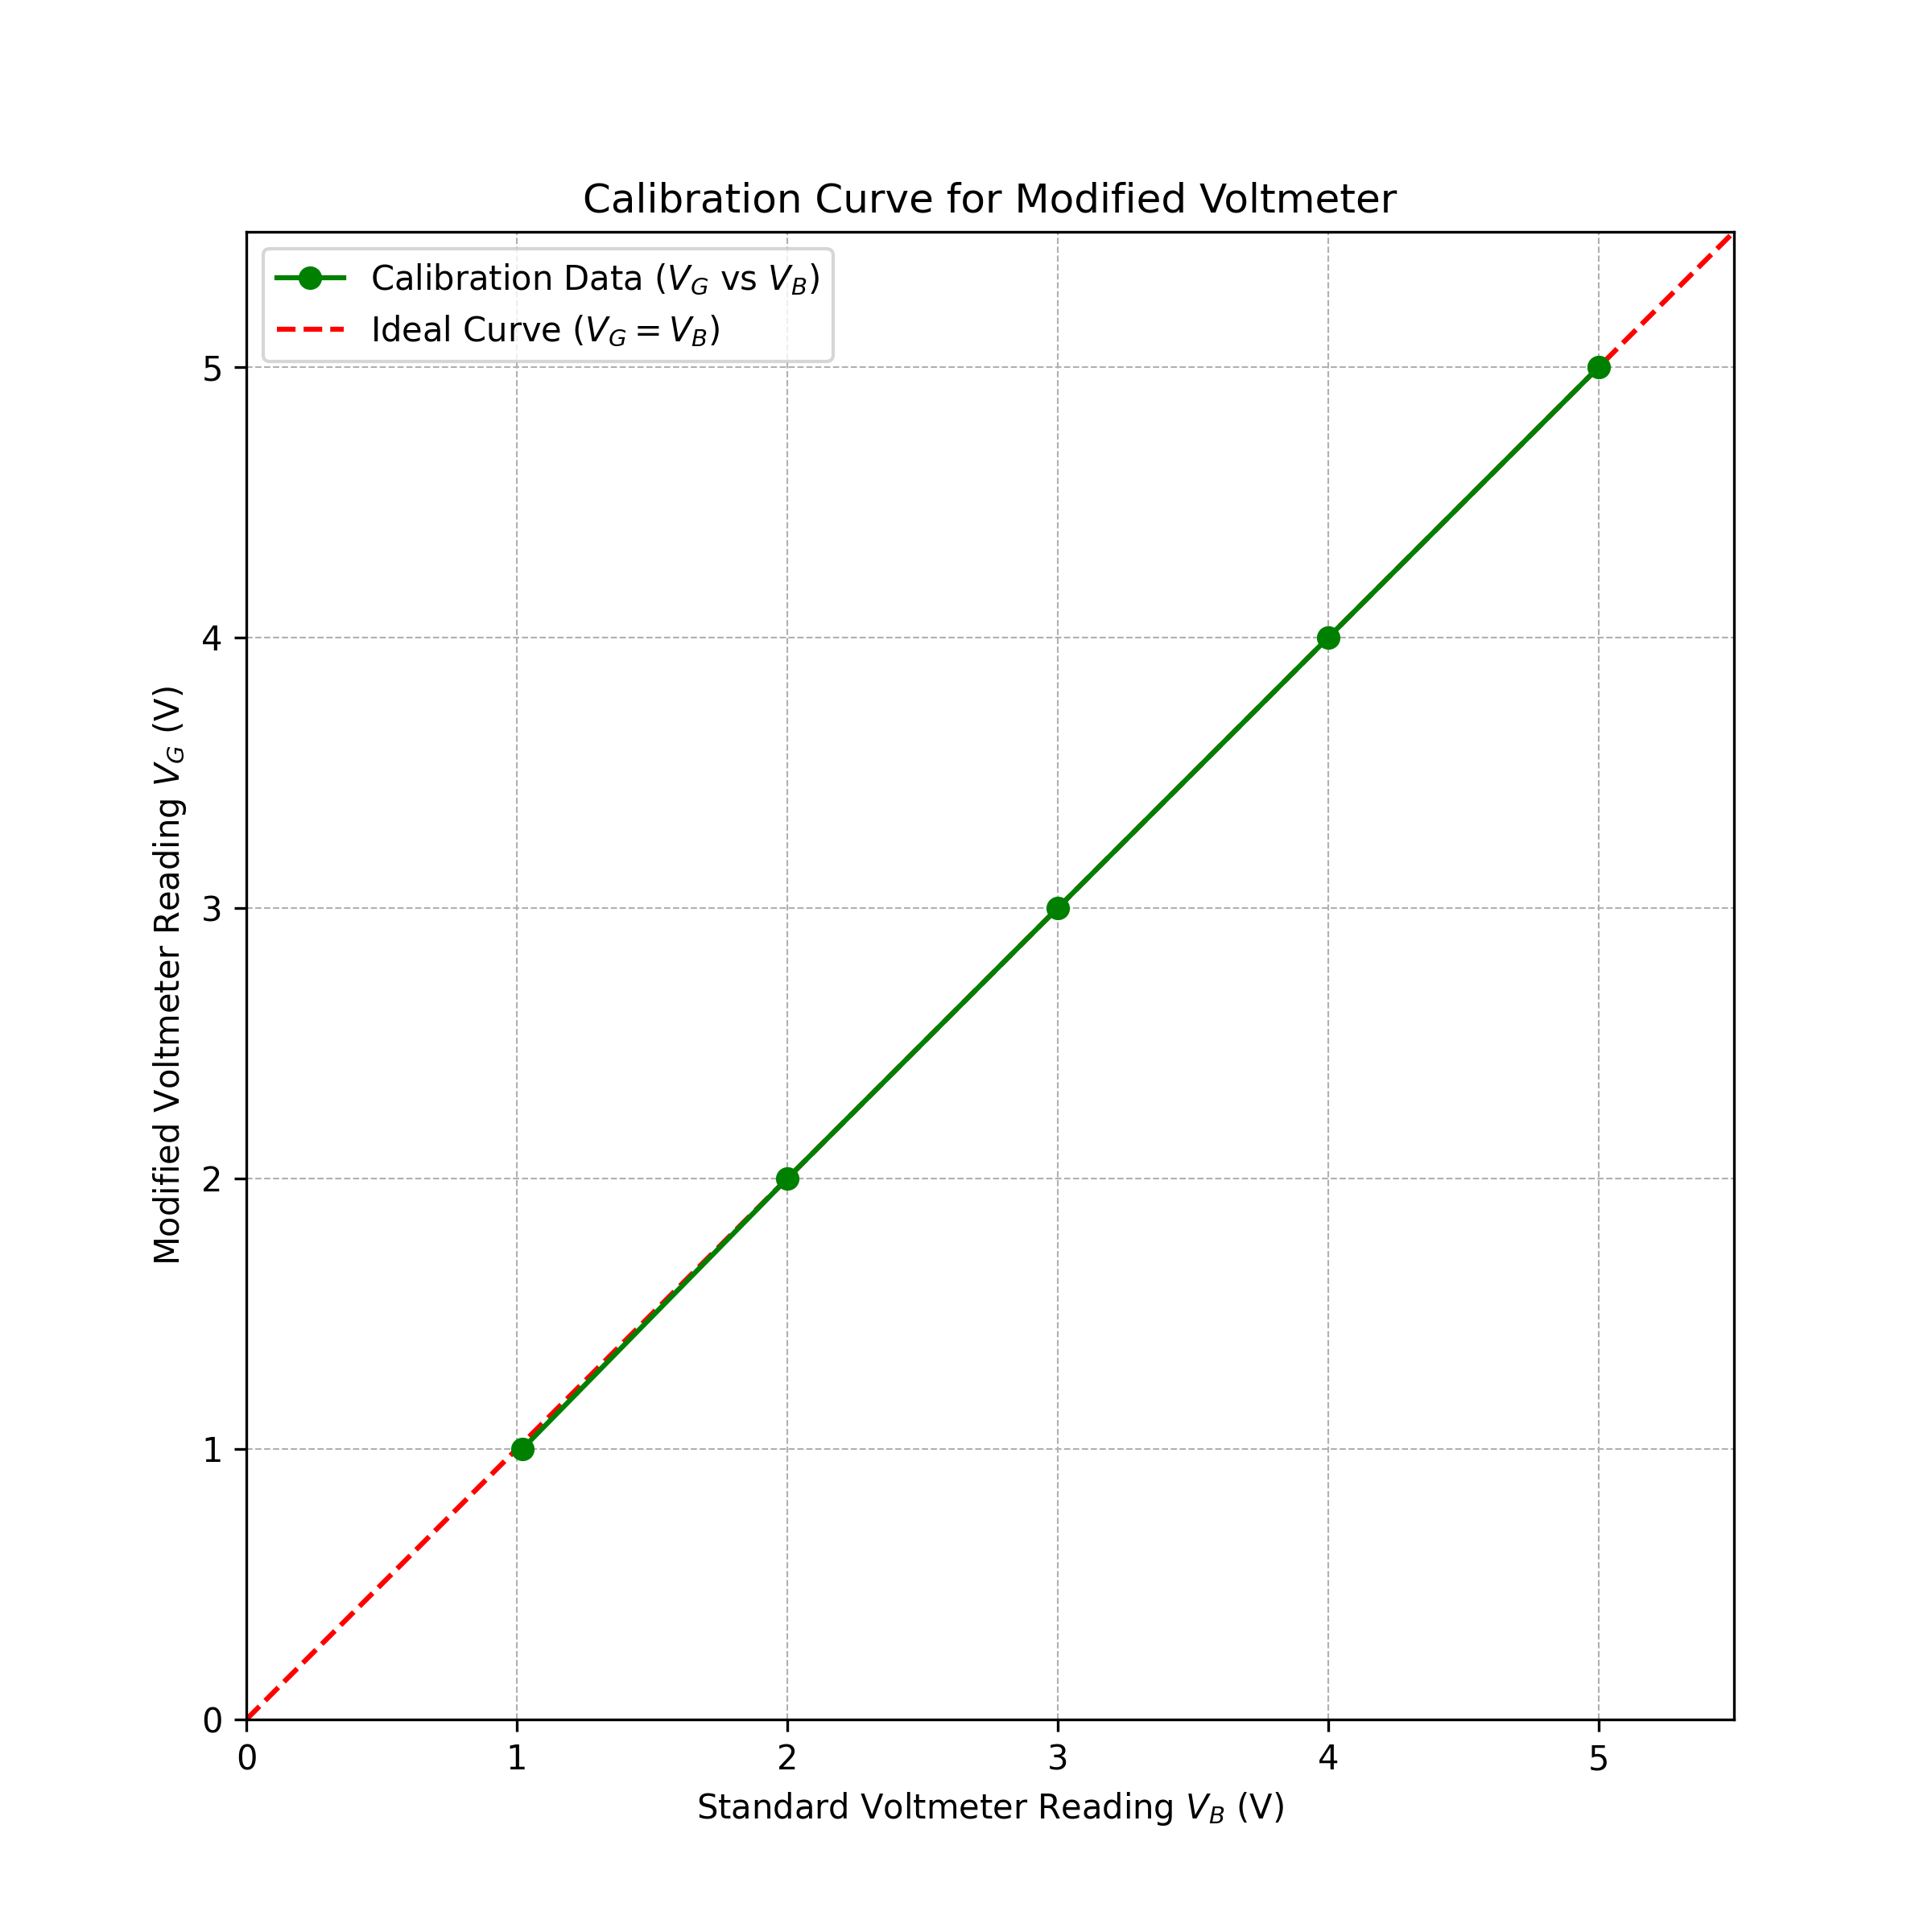
\includegraphics[width=0.4\textwidth]{figure/V.png}
  \caption{改装电压表的$V_G-V_B$曲线}
  \label{graphV}
\end{figure}

\subsubsection{设计并改装欧姆表}
欧姆调零后依次改变欧姆表负载电阻，读出负载电阻对应的欧姆表示数$I_x$和电阻值$R_x$，
记录实验数据如下表所示
\begin{table}[H]
  \centering
  \caption{改装欧姆表的实验数据}
  \begin{tabular}{cccccccccccc}
    \toprule
    实验序号 & 1 & 2 & 3 & 4 & 5 & 6 & 7 & 8 & 9 & 10 &\\
    \midrule
    $I_x({mA})$ & 4.95 & 4.75 & 4.70 & 4.20 & 4.00 & 3.80 & 3.60 & 3.335 & 3.15 & 3.00 \\
    \midrule
    $R_x(\Omega)$ & 1.0 & 10.0 & 20.0 & 50.0 & 70.0 & 90.0 & 110.0 & 140.0 & 160.0 & 180.0 \\
    \bottomrule
    \label{tableOhm}
  \end{tabular}
\end{table}

欧姆表方程为
\[
I_x=\frac{EI_g}{E+I_g R_x}
\]
\begin{figure}[H]
        \centering
        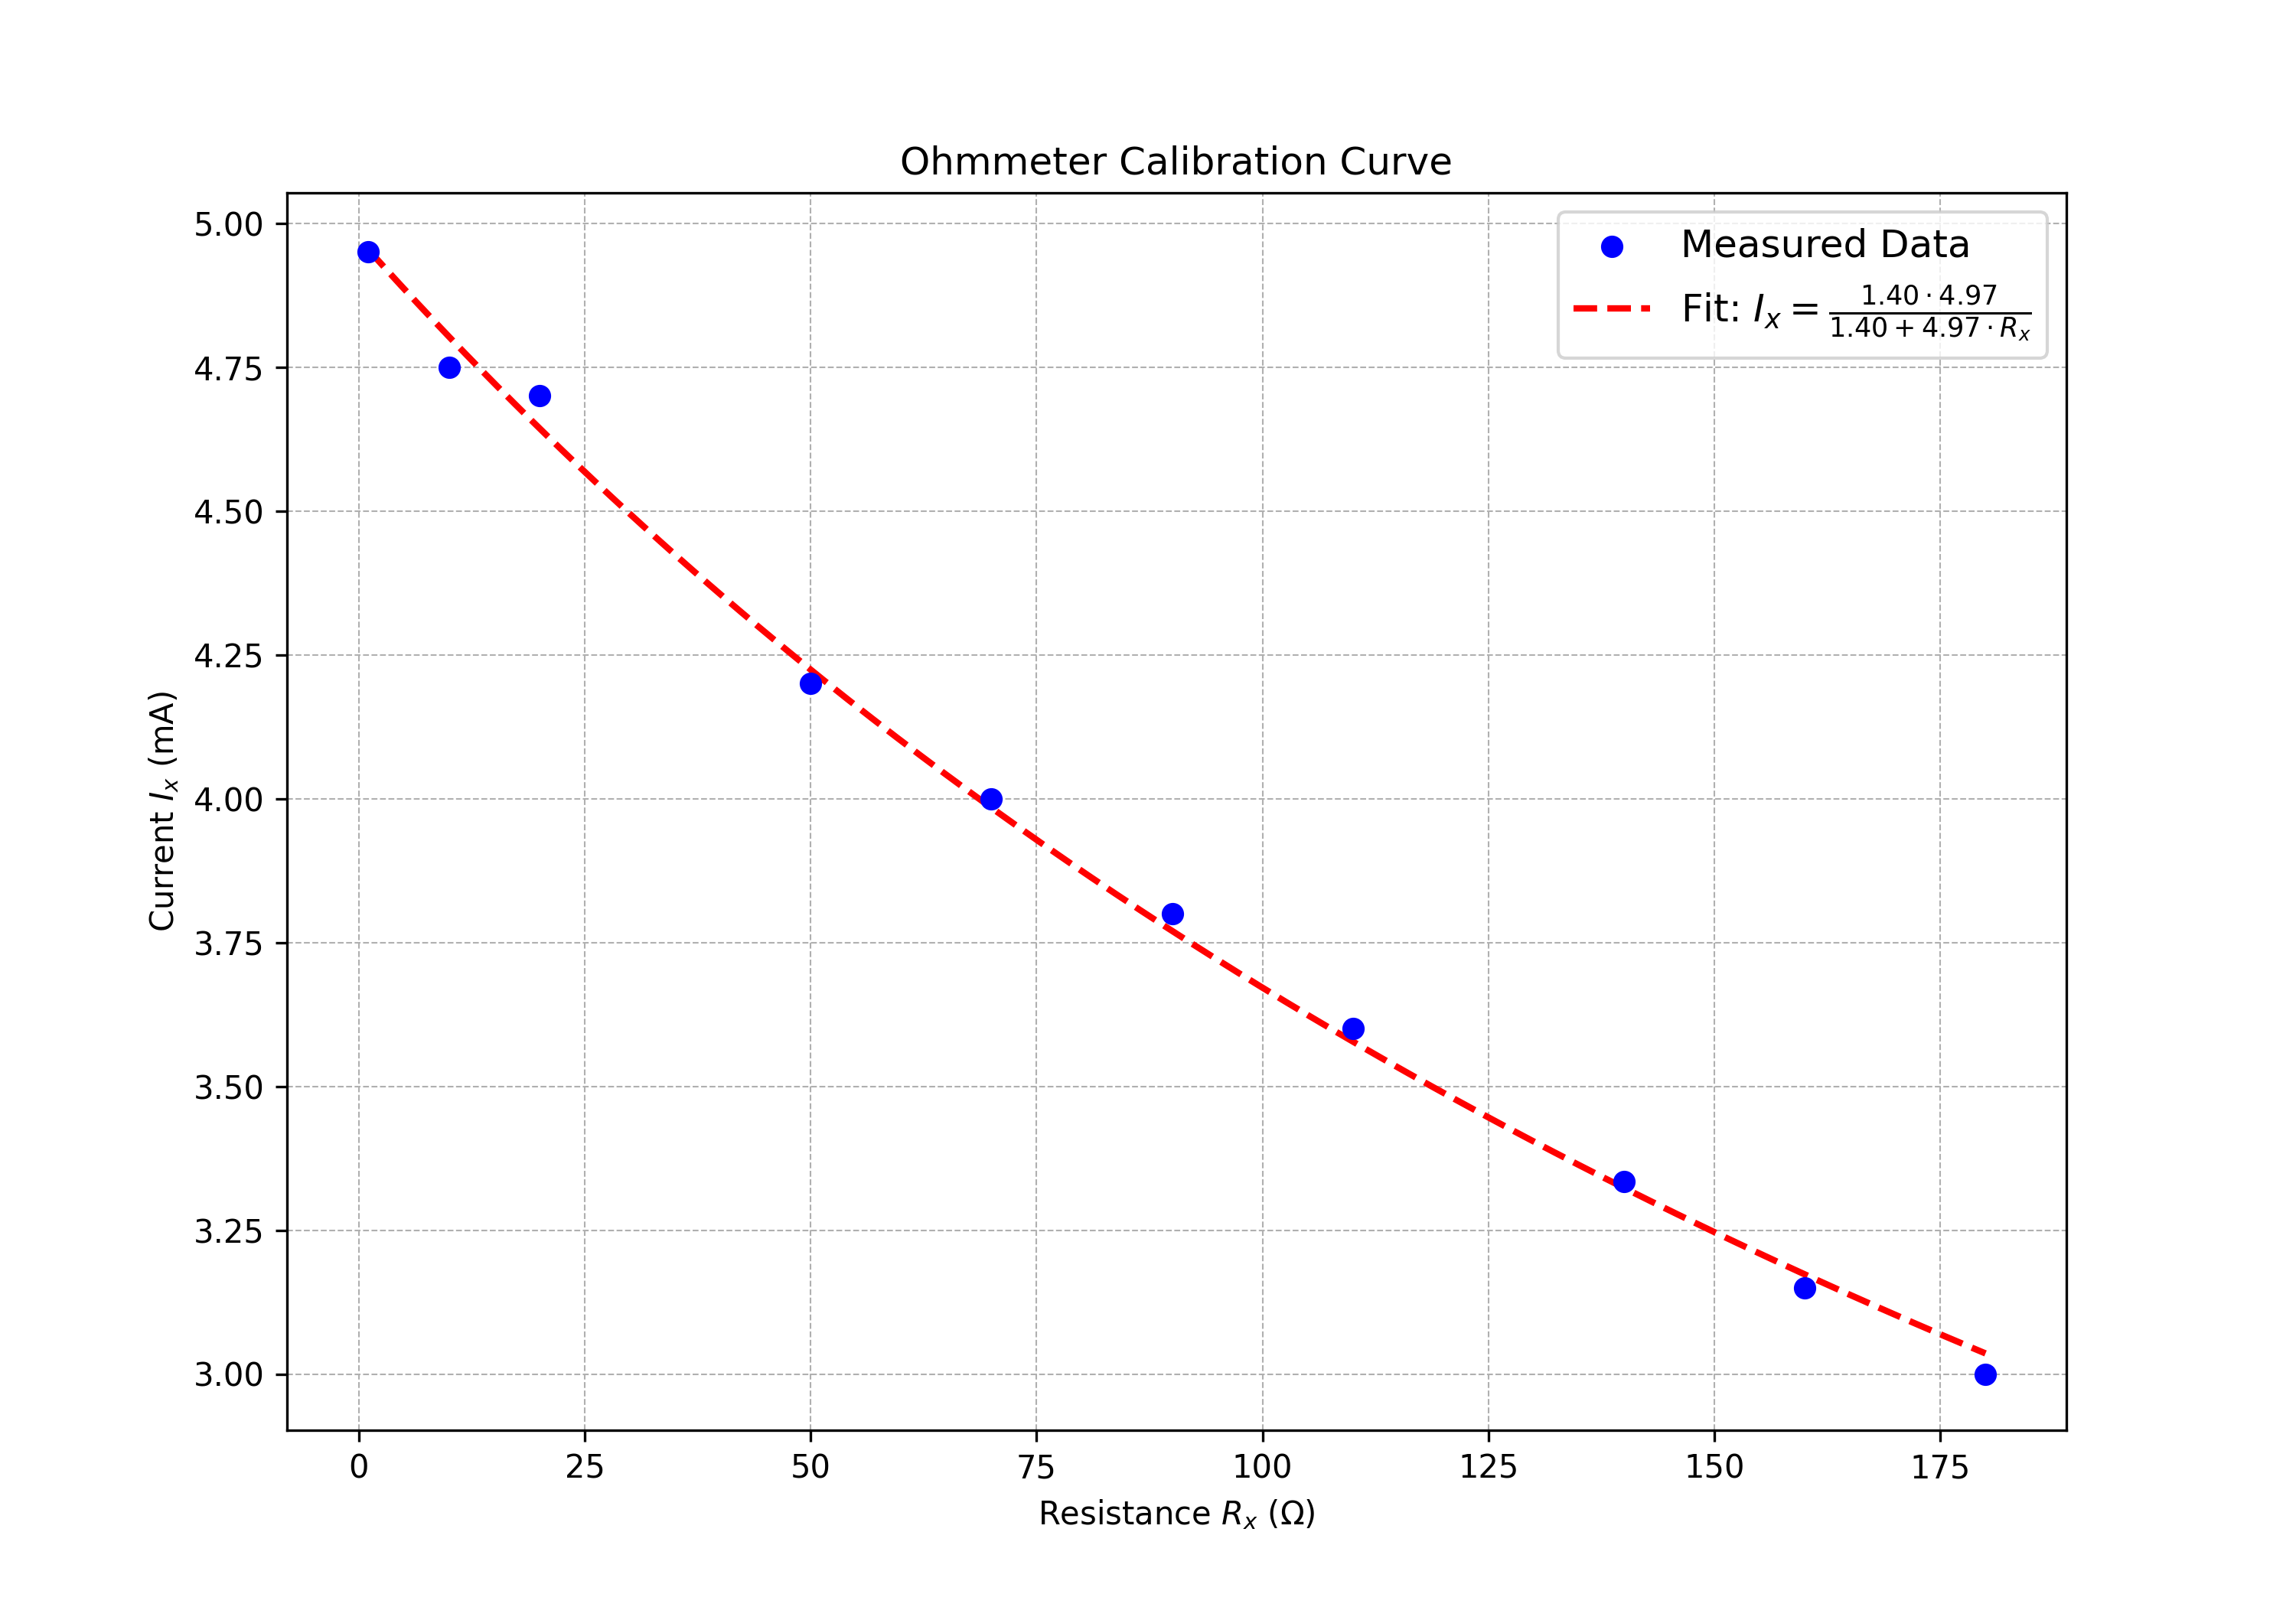
\includegraphics[width=0.4\textwidth]{figure/R.png}
        \caption{改装欧姆表的$I_x-R_x$曲线}
        \label{graphOhm}
\end{figure}
拟合结果显示$E=1.47V$，$I_g=4.97mA$

可见，欧姆表的示数随通过的电流增大非线性地减小，而且，通过的电流越大，减小的速率就越缓。
即，在欧姆表表盘上，最大电流刻度为0，最小电流刻度为$\infty$，
从右往左电阻示数依次增大；电阻间隔一致时，刻度间隔左密右疏。

    \myspace{2}
\subsection{误差分析}
    \xiaosi （运用测量误差、相对误差、不确定度等分析实验结果，20分）

\textbf{1. 系统误差}
\begin{itemize}
    \item \textbf{电表内阻测量误差}：替代法测量内阻时，开关接触电阻、导线电阻等引入系统误差，导致$R_g$的测量值不准确。
    \item \textbf{电阻箱精度误差}：使用的电阻箱具有最小步进值，其实际阻值与标称值存在偏差，影响改装精度。
    \item \textbf{电源电动势变化}：实验过程中电池电动势存在微小变化，特别是在欧姆表测量中，电源内阻和电动势的波动直接影响测量结果。
    \item \textbf{标准表误差}：用于校准的标准表本身存在一定的精度等级限制，引入系统误差。
\end{itemize}

\textbf{2. 随机误差}
\begin{itemize}
    \item \textbf{读数误差}：指针式电表读数时存在视差，数字表最后一位存在跳动。
    \item \textbf{环境因素}：温度变化影响电阻阻值，特别是金属膜电阻的温度系数不可忽略。
    \item \textbf{接触电阻不稳定}：接线柱、开关等接触部位电阻随时间变化。
\end{itemize}

\textbf{3. 电表等级误差分析}
\begin{itemize}
    \item 电流表引用误差1.0\%，达到1.0级标准。主要误差来源为分流电阻的选取和校准过程中的读数误差。
    \item 电压表引用误差0.4\%，评定为0.5级。串联电阻的阻值调整是影响精度的关键因素。
    \item 欧姆表的非线性特性导致测量误差分布不均匀，中值电阻附近精度最高，两端误差增大。
\end{itemize}

    \subsection{实验探讨}
    \xiaosi （对实验内容、现象和过程的小结，不超过100字，10分）

    本实验通过实际动手操作，深入理解了电表改装的原理和方法。实验过程中发现，电表内阻的精确测量是成功改装的基础，而电阻的选取和校准直接决定了改装后电表的精度等级。欧姆表的非线性刻度特性使其在测量不同范围电阻时精度差异显著，实际操作中应尽量使待测电阻值接近中值电阻以提高测量精度。通过本次实验，不仅掌握了万用表各档位的设计原理，还培养了电路设计、误差分析和仪器调试的综合能力。

\section{思考题}

    \xiaosi （解答教材或讲义或老师布置的思考题，10分）
    
1、为什么不能用万用表欧姆档测量电源内阻？

万用表的欧姆档工作原理是在被测电阻两端施加一个已知的测试电压，通过测量流过电阻的电流来计算阻值。当用欧姆档测量电源内阻时：
电源本身具有电动势，会叠加在万用表的测试电压上，导致测量电流不准确。
可能产生大电流，损坏万用表的欧姆档测量电路。
电源内阻通常很小（几欧姆到几十欧姆），而万用表欧姆档的低阻值测量精度有限。

正确的方法应采用伏安法或电桥法测量电源内阻。

2、为什么不能用欧姆表测量另一表头内阻？

主要原因如下：
\begin{itemize}
    \item 欧姆表工作时需要向被测电阻提供电流，而表头允许通过的电流非常有限（通常为微安级或毫安级），欧姆表提供的测试电流可能超过表头的最大允许电流，导致表头损坏。
    \item 表头内部有游丝等精密部件，过大的电流会使其过热或产生永久形变。
    \item 欧姆表的测试电压可能超过表头的绝缘耐压值。
\end{itemize}
测量表头内阻应采用小电流的测量方法，如电桥法或替代法。

3、为什么$I_x$与$R_x$为非线性关系？

根据欧姆表的基本方程：
\[
I_x = \frac{E I_g}{E + I_g R_x}
\]
这是一个反比例函数关系，其非线性特性源于：
\begin{itemize}
    \item 分母中的$I_g R_x$项使得$I_x$与$R_x$不呈简单的反比关系。
    \item 对$I_x$求关于$R_x$的导数：
    \[
    \frac{dI_x}{dR_x} = -\frac{E I_g^2}{(E + I_g R_x)^2}
    \]
    该导数本身是$R_x$的函数，说明$I_x$的变化率随$R_x$变化。
    \item 二阶导数：
    \[
    \frac{d^2I_x}{dR_x^2} = \frac{2E I_g^3}{(E + I_g R_x)^3} > 0
    \]
    表明曲线下凸，随着$R_x$增大，$I_x$减小的速度逐渐变缓。
\end{itemize}
这种非线性关系导致了欧姆表刻度的不均匀性：低阻值区域刻度稀疏，高阻值区域刻度密集。

\newpage

hao\textbf{注意事项：}
\xiaosi
\begin{enumerate}
    \item 用PDF格式上传“实验报告”，文件名：学生姓名+学号+实验名称+周次。
    \item  “实验报告”必须递交在“学在浙大”的本课程的对应实验项目的“作业”模块内。
    \item  “实验报告”成绩必须在“浙江大学物理实验教学中心网站”-“选课系统”内查询。
    \item 教学评价必须在“浙江大学物理实验教学中心网站”-“选课系统”内进行，学生必须进行教学评价，才能看到实验报告成绩，教学评价必须在本次实验结束后 3 天内进行。
\end{enumerate}

\vspace{1cm}
\xiaosi\centering \textbf{浙江大学物理实验教学中心制}

\end{document}